\section{Diseño}

\subsection{planteamiento de circuito}
Como se menciono anteriormente, utilizando el modulo de matriz de leds MD\_7219.
Utilizando el microcontrolador Arduino Uno, utilizando las entradas digitales se debe 
colocar que lean los botones, siendo este uno rojo y azul. El botón rojo debe hacer que la matriz 
incremente en uno el contador que se lleva hasta llegar a F, si se pasa de F este debe volver a 0. El botón
azul debe hacer que la cuenta disminuya por cada toque hasta llegar a 0, si este se presiona nuevamente se debe
regresar a F. Teniendo el anterior planteamiento y conectando el modulo directo a la placa, con la alimentación
de $\SI{5}{\volt}$ y a tierra, se tiene el siguiente diagrama:
\begin{figure}[h!]
    \centering
    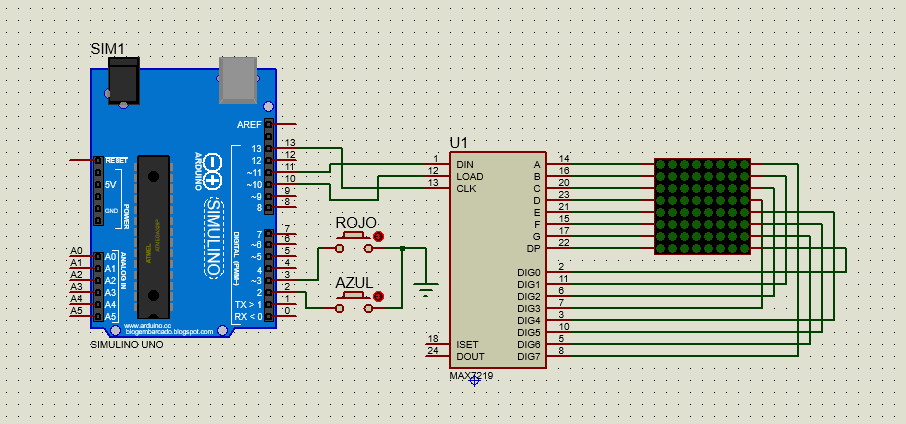
\includegraphics[width=0.8\textwidth]{Diagramas/Diagrama.png}
    \caption{Diagrama de conexión}
    \label{fig:conexion}
\end{figure}

Ahora bien, ya que el modulo no existe en el simulador, se construyo utilizando el circuito integrado y una matriz de leds
entregadas por el programa. Igualmente, se observan ambos botones conectados a tierra. Estos botones, están en configuración
de pull up, osea que los pines están energizados en $\SI{5}{\volt}$ mediante una resistencia de pull up, entregando el valor HIGH,
si se presiona el botón, este pasa a LOW, teniendo asi las entradas digitales de nuestro montaje. Para la salida de nuestro circuito 
se tiene la matriz construido, asi esta se tiene que conectar a un voltaje de alimentación y a tierra, pero en proteus no se puede realizar esto, 
pero teniendo considerado esto para la implementación del circuito.

\subsection{Desarrollo del código}
Para el desarrollo del código que se implementa en el Arduino Uno, se utilizo la biblioteca \texttt{MD\_MAX72xx}, se uso
el recurso \cite{programarfacilMax7219} para aprender de los comandos de la biblioteca. Y la biblioteca \texttt{SPI} para 
la comunicación entre el modulo y el Arduino Uno. Asi el código hecho se observa en \autoref{lst:cod-1}. A continuación, se explicara 
bloque a bloque la lógica de este.
\clearpage
\begin{listing}[H]
    \begin{minted}{cpp}
        #include <MD_MAX72xx.h>
        #include <SPI.h>

        #define hardware MD_MAX72XX::GENERIC_HW
        #define pinDIN 11
        #define pinCS 10
        #define pinCLK 13

        MD_MAX72XX mx = MD_MAX72XX(hardware,pinDIN,pinCLK,pinCS,1);

        const int botonPin1 = 3;  
        const int botonPin2 = 2;
        int contador = 0;         
        int estadoAnterior = HIGH; 
        int estadoAnterior2 = HIGH;
    \end{minted}
    \caption{Definición de variables}
    \label{lst:b1}
\end{listing}

Como se menciono anteriormente, las bibliotecas utilizadas sirven para comunicarse y controlar el modulo. Ahora bien en \autoref{lst:b1},
primero se definieron los pines y el hardware utilizado en este caso, siendo el genérico, para luego definir un objeto
\texttt{mx} con las especificaciones definidas en las lineas anteriores.   

\begin{listing}[H]
    \begin{minted}{cpp}
        void setup() {
            mx.begin();

            mx.setChar(5,'0');
            pinMode(botonPin1, INPUT_PULLUP); 
            pinMode(botonPin2, INPUT_PULLUP);
            Serial.begin(9600);
        }
    \end{minted}
    \caption{Setup del código}
    \label{lst:b2}
\end{listing}
En \autoref{lst:b2}, se inicia la matriz de leds y los pines definidos en \autoref{lst:b1}, cabe destacar que en el diseño se consideraron estos botones
de Pull up, para esto se tendría que colocar una resistencia, pero el Arduino Uno posee esta resistencia en el pin, utilizando \texttt{INPUT\_PULLUP} esta se activa.
Una vez iniciado el circuito este mostrara siempre el cero al incoo como se observa en el bloque. Por ultimo, se inicia la comunicación
serial a $\SI{9600}{\frac{\bit}{\second}}$.

\clearpage
Para la parte de \texttt{loop()}, se separara en dos partes la explicación de este, una parte para el boton rojo y otro para el boton azul. Para el primer boton, se tiene:

\begin{listing}[H]
    \begin{minted}{cpp}
        int estadoActual = digitalRead(botonPin1);
        if (estadoAnterior == HIGH && estadoActual == LOW) {
            mx.clear();
            contador++;
            if(contador>15) contador = 0;
            if (contador <= 9){
                mx.setChar(5,'0'+contador);
            }
            else if (contador>=10 && contador<=15){
            mx.setChar(5,'7'+ contador);
            }
    
            Serial.println(contador);
            delay(200); 
        }
        estadoAnterior = estadoActual; 
    \end{minted}
\end{listing}